%卒論概要テンプレート ver. 3.0

\documentclass[uplatex,twocolumn,dvipdfmx]{jsarticle}
\usepackage[top=22mm,bottom=22mm,left=22mm,right=22mm]{geometry}
\setlength{\columnsep}{10mm}
\usepackage[T1]{fontenc}
\usepackage{txfonts}
\usepackage[expert,deluxe]{otf}
\usepackage[dvipdfmx,hiresbb]{graphicx}
\usepackage[dvipdfmx]{hyperref}
\usepackage{pxjahyper}
\usepackage{secdot}





%タイトルと学生番号,名前だけ編集すること
\title{\vspace{-5mm}\fontsize{14pt}{0pt}\selectfont 調達資金の時間変化測定に基づくクラウドファンディングの成功要因分析}
\author{\normalsize プロジェクトマネジメントコース 矢吹研究室 1342066 島田樹}
\date{}
\pagestyle{empty}
\begin{document}
\fontsize{10.5pt}{\baselineskip}\selectfont
\maketitle





%以下が本文
\section{序論}
クラウドファンディングとは,自らのアイディアやプロジェクトをネット上でプレゼンテーションすることで,支援者を集めて資金を獲得する手法である.SNSの発達に伴いプロジェクトの数も増加し,市場も年々増加している\cite{visualizing}.幅広い分野と規模での応募が可能で,ベンチャー企業のプロジェクトや学生の研究費用の獲得などが多かったが,大手企業も支援者数から売れることを確実視されたプロダクトを販売者できるとして,マーケティングの一環として活用されるようになってきた.

課題研究において,調達資金の時間変化を調査し可視化したところ,資金が集まり始める時期には実行者が何らかの行動をしていると考えた.資金が集まる直前の実行者の行動を分析すればクラウドファンディングにおけるプロジェクトの成功率を上げることができるのではないかと考えた.


\section{目的}
先行研究\cite{miura}ではプロジェクトの内容以外の要因を調査し,目標金額等の設定段階で成功率を上げることを目的としていた.本研究では調達資金の時間変化を可視化し,動画の投稿やSNSでの告知などの多くの資金を集める直前に行っているプロジェクト実行者の行動を分析する.その結果から,プロジェクト実行者が資金を集める際の参考となる指標を作ることを目的とする.


\section{手法}
初めにクラウドファンディングサイトを,毎日定時に監視し,データ収集を行う.収集したデータから成功しているプロジェクトの資金調達を可視化し,資金が集まり始めるときにしている行動を調査する.調査項目は,サイト内のレポートを活用しているか,動画を投稿しているか,Twitterでツイートをしているか,Facebookで投稿しているか,の4項目である.この4項目に調達金額を目標金額で割った目標達成率を足した5項目から決定木を作成し,調達資金に必要な行動を考察する.


\section{結果}
決定木分析結果が図1である.目標達成率を目的変数とおいて,レポートとツイートが最も資金調達に関係が深い説明変数となった.

\begin{figure}[h]
\centering
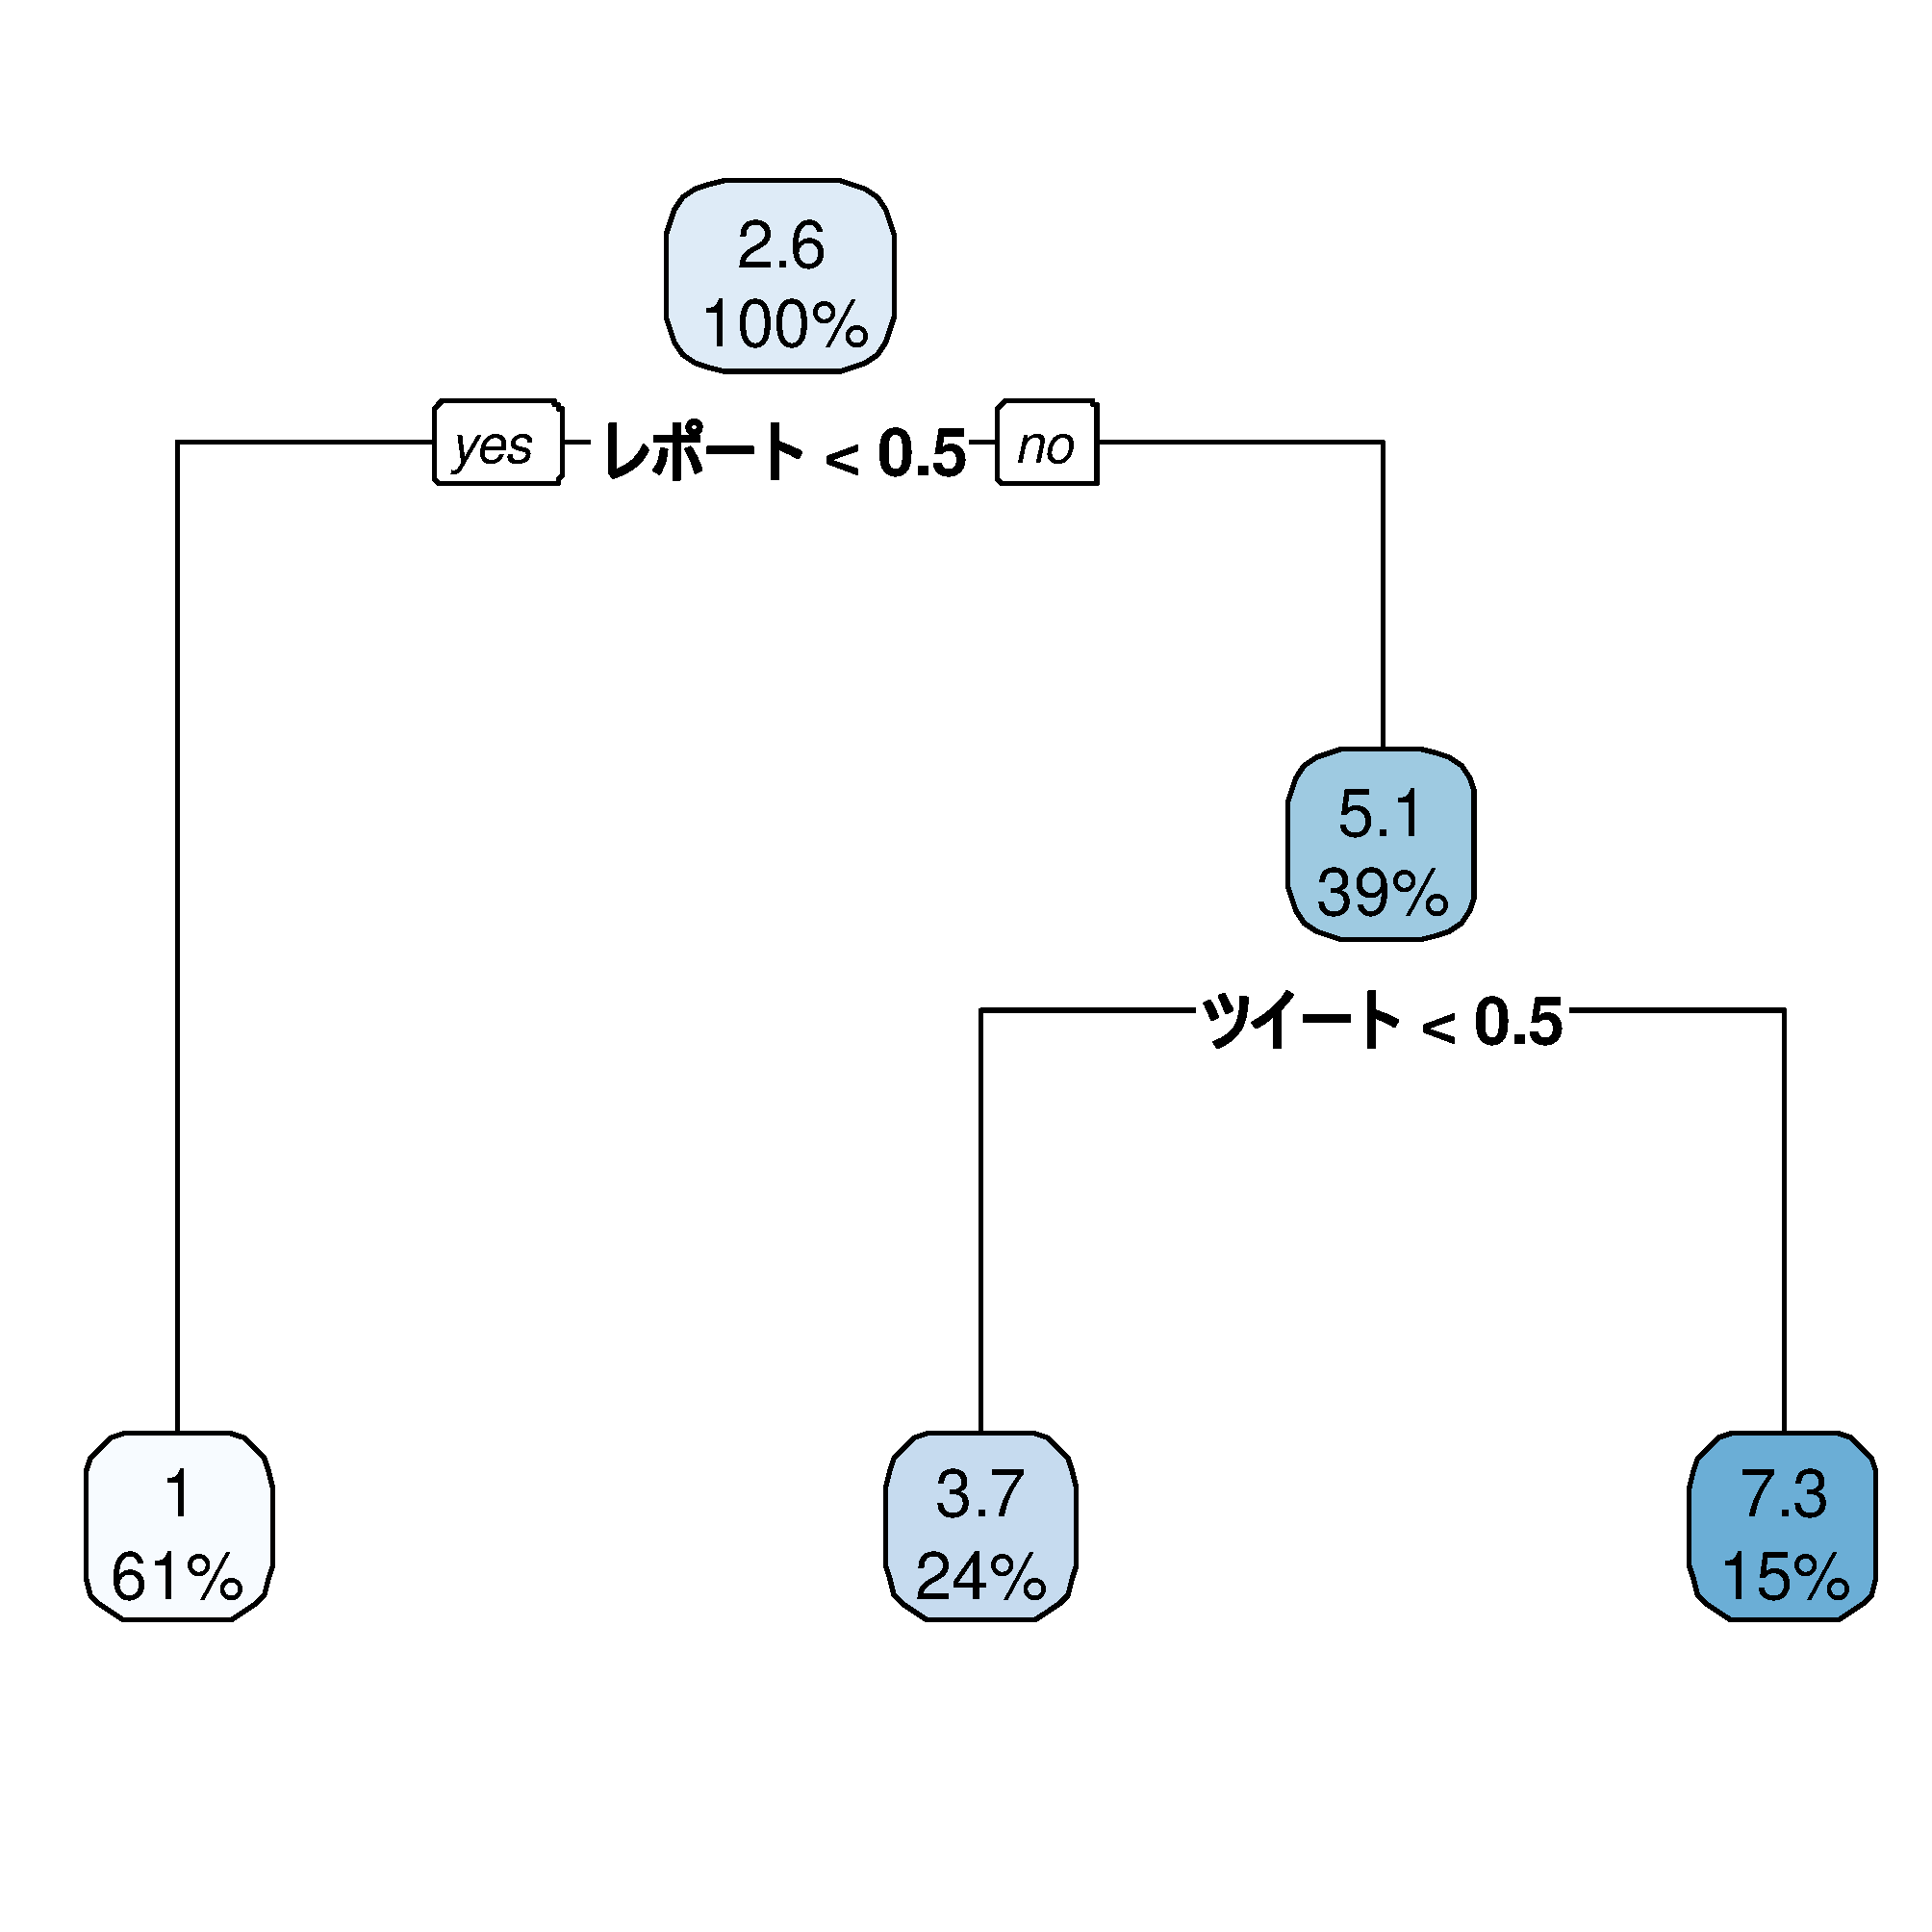
\includegraphics[width=4.2cm,clip]{ket.pdf}
\caption{目標達成率に対する決定木分析}\label{サンプル図}
\end{figure}

\section{考察}
図1から,レポートとツイートをしてるプロジェクトが資金の調達に最も成功していることがわかる.レポートはプロジェクトのページからすぐに閲覧可能なため,支援者の目につきやすいからだと考えられる.ツイートに関しては,情報の拡散力の高いTwitterによって多数の支援者の目に留まり資金が集まったと考えられる.


\section{結論}
本研究で,クラウドファンディングにおいて資金調達する際にプロジェクト実行者がするべき行動はレポートとツイートであるという結果が出た.上記の項目以外に資金調達に関係があると思われる項目を増やしていくことで,さらに精度の高い結果を得られるはずだ.

\bibliographystyle{junsrt}
\bibliography{biblio}%「biblio.bib」というファイルが必要.

\end{document}
